\Chapter{Tesztelés}

Ebben a fejezetben kerülnek bemutatásra az alkalmazáshoz készült automatikus, illetve manuális tesztek.

\Section{Automatikus tesztek}

Modern webalkalmazás lévén esetünkben is elengedhetetlen az automatikus tesztelés. Minden egyes funkcióhoz készültek egységtesztek, melyek biztosítják a megfelelő működésüket.

Szerveroldalon egyetlen fontos végpont van, amit tesztelni kellett, az pedig a \\
\textit{/api/generate-questions} útvonal.

\begin{figure}[h]
\centering
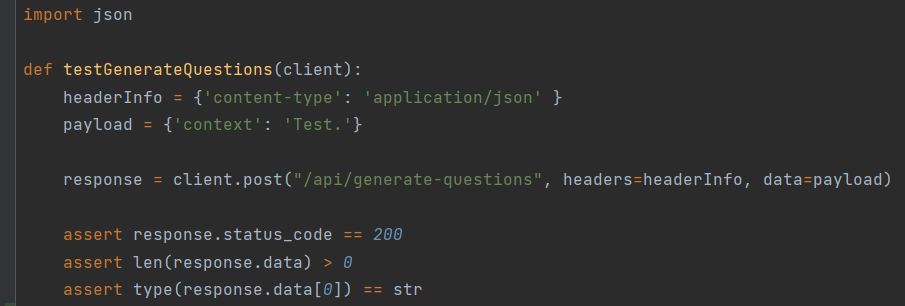
\includegraphics[scale=0.6]{images/test_backend_1.png}
\caption{A szerveroldali végpont egységtesztje.}
\label{fig:tb1}
\end{figure}

A \textbf{qg\_app\_backend} konténerbe terminállal belépve a \textit{pytest} parancs futtatásával lehet elindítani a szerveroldali teszteket. Ekkor minden \textbf{test} szót tartalmazó fájlt tesztnek érzékel és lefuttat a tesztkörnyezet.

\begin{figure}[h]
\centering

\includegraphics[scale=0.5]{images/test_backend_2.png}
\caption{A szerveroldali tesztek eredménye.}
\label{fig:tb2}
\end{figure}

\pagebreak

Kliens oldalon minden komponenshez készült egységteszt, melyek az adott komponenssel egy mappába kerültek elhelyezésre. Készült továbbá néhány integrációs teszt is az egyes oldalakhoz, illetve az alkalmazás egészéhez.

\begin{figure}[h]
\centering
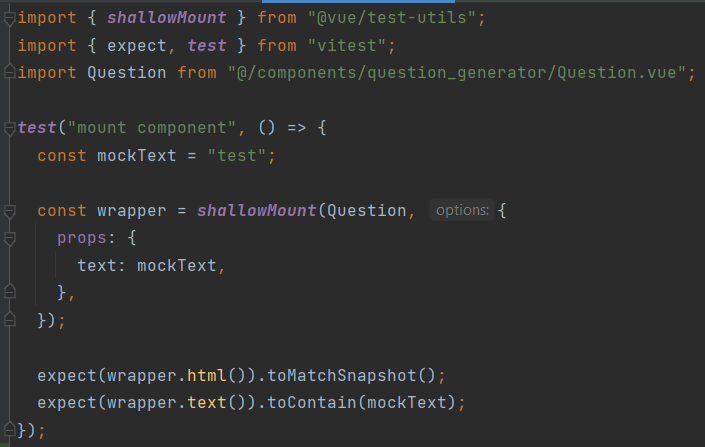
\includegraphics[scale=0.6]{images/test_frontend_1.png}
\caption{Question nevű komponens egységtesztje.}
\label{fig:tf1}
\end{figure}

\begin{figure}[h]
\centering
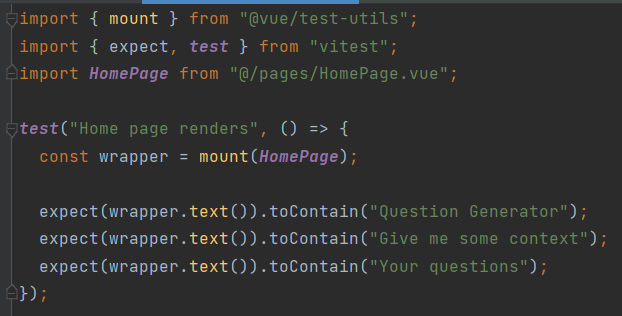
\includegraphics[scale=0.6]{images/test_frontend_2.png}
\caption{A főoldal integrációs tesztje.}
\label{fig:tf2}
\end{figure}

A kliensoldai egységtesztek futtatásához a \textbf{qg\_app\_frontend} konténerbe kell belépnünk és el kell indítanunk a \textit{npm run test} parancsot. Ekkor szintén minden kliensoldali \textbf{test} szót tartalmazó fájlban lefutnak a tesztek.

\pagebreak

\begin{figure}[h]
\centering
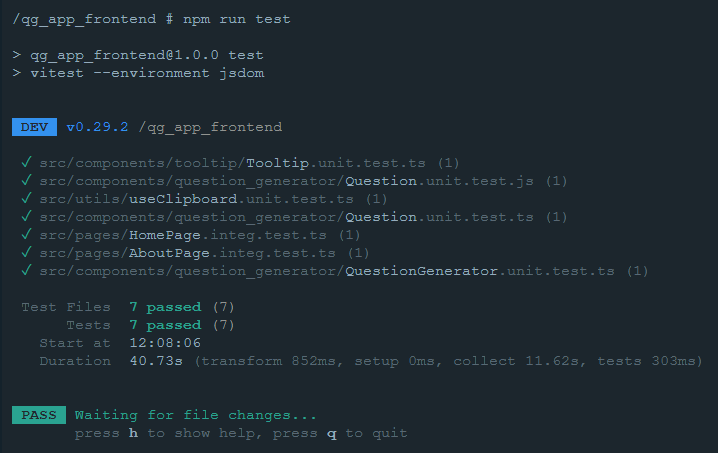
\includegraphics[scale=0.6]{images/test_frontend_3.png}
\caption{A kliensoldali tesztek eredménye.}
\label{fig:tf3}
\end{figure}

\Section{Manuális tesztek}

Mivel alkalmazásunk egy NLP feladat megoldására íródott, így elengedhetetlen, hogy kézzel is teszteljük. Ez esetünkben annyit jelentett, hogy különböző kontextusokat adtunk meg az alkalmazásnak és figyeltük, hogy milyen kérdéseket generált. Egy kérdés akkor számít elfogadottnak, ha értelmes, van köze a kontextushoz és nyelvtanilag is helyes.

\begin{figure}[h]
\centering
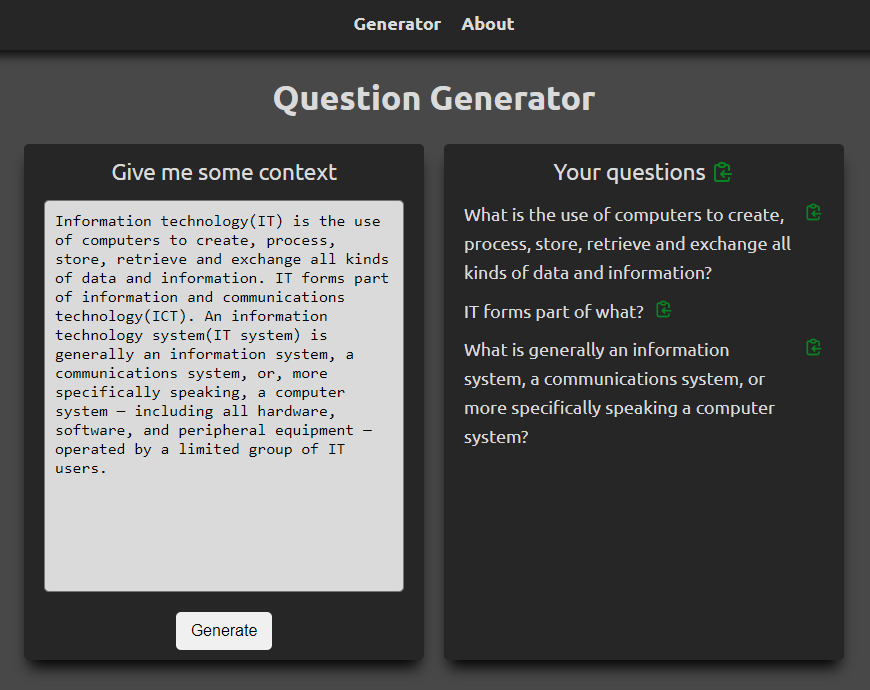
\includegraphics[scale=0.5]{images/test_manual.png}
\caption{Az alkalmazás egy manuális tesztje.}
\label{fig:tm}
\end{figure}

\pagebreak

A kezdeti tesztek elsősorban az alap működés ellenőrzésére szolgáltak, vagyis hogy képes-e az alkalmazás szavakból, mondatokból vagy hosszabb szövegekből kérdéseket generálni.

\begin{itemize}
\item \textbf{Kontextus:} "one"
\item \textbf{Kérdések:} 
	\begin{itemize}
		\item How many questions does one have to answer in order to get a good answer?
	\end{itemize}
\item \textbf{Kontextus:} "hungarian"
\item \textbf{Kérdések: }
	\begin{itemize}
		\item What is the nationality of the hungarian population?
		\item What country is the capital of Hungary?
	\end{itemize}
\item \textbf{Kontextus:} "Hungary is a country."
\item \textbf{Kérdések:}
	\begin{itemize}
		\item What is Hungary?
		\item What is a country?
	\end{itemize}
\item \textbf{Kontextus:} "Kate made an apple pie."
\item \textbf{Kérdések:}
	\begin{itemize}
		\item Kate made what kind of pie?
	\end{itemize}
\item \textbf{Kontextus:} "Information technology(IT) is the use of computers to create, process, store, retrieve and exchange all kinds of data and information. IT forms part of information and communications technology(ICT). An information technology system(IT system) is generally an information system, a communications system, or, more specifically speaking, a computer system — including all hardware, software, and peripheral equipment — operated by a limited group of IT users."
\item \textbf{Kérdések:}
	\begin{itemize}
		\item What is the use of computers to create, process, store, retrieve and exchange all kinds of data and information?
		\item IT forms part of what?
		\item What is generally an information system, a communications system, or more specifically speaking a computer system?
	\end{itemize}
	\item \textbf{Kontextus:} "A transformer is a deep learning model that adopts the mechanism of self-attention, differentially weighting the significance of each part of the input data. It is used primarily in the fields of natural language processing (NLP) and computer vision (CV).
Like recurrent neural networks (RNNs), transformers are designed to process sequential input data, such as natural language, with applications towards tasks such as translation and text summarization. However, unlike RNNs, transformers process the entire input all at once. The attention mechanism provides context for any position in the input sequence. For example, if the input data is a natural language sentence, the transformer does not have to process one word at a time. This allows for more parallelization than RNNs and therefore reduces training times."
\item \textbf{Kérdések:}
	\begin{itemize}
		\item What is a deep learning model that adopts the mechanism of self-attention?
		\item What is used primarily in the fields of natural language processing (NLP) and computer vision (CV)?
		\item Like recurrent neural networks, transformers are designed to process what input data?
	\end{itemize}
\end{itemize}

Ezt követően elkezdtünk az alkalmazásnak különböző témakörökből kontextusokat megadni, hiszen célunk, hogy minél színesebb témaválasztékból tudjon a program kérdéseket generálni.

\begin{itemize}
\item \textbf{Témakör:} Fizika
\item \textbf{Kontextus:} "The Schrödinger equation is a linear partial differential equation that governs the wave function of a quantum-mechanical system. It is a key result in quantum mechanics, and its discovery was a significant landmark in the development of the subject. The equation is named after Erwin Schrödinger, who postulated the equation in 1925, and published it in 1926, forming the basis for the work that resulted in his Nobel Prize in Physics in 1933.
Conceptually, the Schrödinger equation is the quantum counterpart of Newton's second law in classical mechanics. Given a set of known initial conditions, Newton's second law makes a mathematical prediction as to what path a given physical system will take over time. The Schrödinger equation gives the evolution over time of a wave function, the quantum-mechanical characterization of an isolated physical system. The equation can be derived from the fact that the time-evolution operator must be unitary, and must therefore be generated by the exponential of a self-adjoint operator, which is the quantum Hamiltonian.
The Schrödinger equation is not the only way to study quantum mechanical systems and make predictions. The other formulations of quantum mechanics include matrix mechanics, introduced by Werner Heisenberg, and the path integral formulation, developed chiefly by Richard Feynman. Paul Dirac incorporated matrix mechanics and the Schrödinger equation into a single formulation. When these approaches are compared, the use of the Schrödinger equation is sometimes called "wave mechanics"."
\item \textbf{Kérdések:} 
	\begin{itemize}
		\item What is a linear partial differential equation that governs the wave function of a quantum-mechanical system?
		\item Who is the Schrödinger equation named after?
		\item What is the quantum counterpart of Newton's second law in classical mechanics?
		\item Which formulation of quantum mechanics was developed by Richard Feynman?
	\end{itemize}
\item \textbf{Témakör:} Történelem
\item \textbf{Kontextus:} "Hungary in its modern (post-1946) borders roughly corresponds to the Great Hungarian Plain (the Pannonian Basin). During the Iron Age, it was located at the crossroads between the cultural spheres of the Celtic tribes (such as the Scordisci, Boii and Veneti), Dalmatian tribes (such as the Dalmatae, Histri and Liburni) and the Germanic tribes (such as the Lugii and Marcomanni). The name "Pannonian" comes from Pannonia, a province of the Roman Empire. Only the western part of the territory (the so-called Transdanubia) of modern Hungary formed part of Pannonia. The Roman control collapsed with the Hunnic invasions of 370–410, and Pannonia was part of the Ostrogothic Kingdom during the late 5th to mid 6th century, succeeded by the Avar Khaganate (6th to 9th centuries). The Magyar invasion took place during the 9th century. The Magyars were Christianized at the end of the 10th century, and the Christian Kingdom of Hungary was established in 1000 under King Saint Stephen, ruled by the Árpád dynasty for the following three centuries. In the high medieval period, the kingdom expanded to the Adriatic coast and entered a personal union with Croatia during the reign of King Coloman in 1102. In 1241 during the reign of King Béla IV, Hungary was invaded by the Mongols under Batu Khan. The outnumbered Hungarians were decisively defeated at the Battle of Mohi by the Mongol army. In this invasion more than 500,000 Hungarian people were massacred and the whole kingdom reduced to ashes. The paternal lineage of the ruling Árpád dynasty came to end in 1301, and all of the subsequent kings of Hungary (with the exception of King Matthias Corvinus) were cognatic descendants of the Árpád dynasty. Hungary bore the brunt of the Ottoman wars in Europe during the 15th century. The peak of this struggle took place during the reign of Matthias Corvinus (r. 1458–1490). The Ottoman–Hungarian wars concluded in significant loss of territory and the partition of the kingdom after the Battle of Mohács of 1526."
\item \textbf{Kérdések:} 
	\begin{itemize}
		\item What is the Pannonian Basin?
		\item Who invaded Hungary in 1241?
		\item How many people were massacred in the Battle of Mohi?
		\item When did the Ottoman-Hungarian wars end?
	\end{itemize}
\item \textbf{Témakör:} Biológia
\item \textbf{Kontextus:} "A virus is a submicroscopic infectious agent that replicates only inside the living cells of an organism. Viruses infect all life forms, from animals and plants to microorganisms, including bacteria and archaea. Since Dmitri Ivanovsky's 1892 article describing a non-bacterial pathogen infecting tobacco plants and the discovery of the tobacco mosaic virus by Martinus Beijerinck in 1898, more than 9,000 of the millions of virus species have been described in detail. Viruses are found in almost every ecosystem on Earth and are the most numerous type of biological entity. The study of viruses is known as virology, a subspeciality of microbiology. When infected, a host cell is often forced to rapidly produce thousands of copies of the original virus. When not inside an infected cell or in the process of infecting a cell, viruses exist in the form of independent viral particles, or virions, consisting of the genetic material, i.e., long molecules of DNA or RNA that encode the structure of the proteins by which the virus acts; a protein coat, the capsid, which surrounds and protects the genetic material; and in some cases  an outside envelope of lipids. The shapes of these virus particles range from simple helical and icosahedral forms to more complex structures. Most virus species have virions too small to be seen with an optical microscope and are one-hundredth the size of most bacteria. The origins of viruses in the evolutionary history of life are unclear: some may have evolved from plasmids—pieces of DNA that can move between cells—while others may have evolved from bacteria. In evolution, viruses are an important means of horizontal gene transfer, which increases genetic diversity in a way analogous to sexual reproduction. Viruses are considered by some biologists to be a life form, because they carry genetic material, reproduce, and evolve through natural selection, although they lack the key characteristics, such as cell structure, that are generally considered necessary criteria for defining life. Because they possess some but not all such qualities, viruses have been described as "organisms at the edge of life" and as replicators."
\item \textbf{Kérdések:} 
	\begin{itemize}
		\item What is a submicroscopic infectious agent that replicates only inside the living cells of an organism?
		\item How many of the millions of virus species have been described in detail since Dmitri Ivanovsky's 1892 article?
		\item What is the study of viruses known as?
	\end{itemize}
\item \textbf{Témakör:} Informatika
\item \textbf{Kontextus:} "In computing, a server is a piece of computer hardware or software (computer program) that provides functionality for other programs or devices, called "clients." This architecture is called the client–server model. Servers can provide various functionalities, often called "services," such as sharing data or resources among multiple clients or performing computations for a client. A single server can serve multiple clients, and a single client can use multiple servers. A client process may run on the same device or may connect over a network to a server on a different device. Typical servers are database servers, file servers, mail servers, print servers, web servers, game servers, and application servers. Client–server systems are usually most frequently implemented by (and often identified with) the request–response model: a client sends a request to the server, which performs some action and sends a response back to the client, typically with a result or acknowledgment. Designating a computer as "server-class hardware" implies that it is specialized for running servers on it. This often implies that it is more powerful and reliable than standard personal computers, but alternatively, large computing clusters may be composed of many relatively simple, replaceable server components."
\item \textbf{Kérdések:} 
	\begin{itemize}
		\item What is a piece of computer hardware or software that provides functionality for other programs or devices called?
		\item What architecture is called the client-server model?
		\item Servers can provide various functionalities, often called what?
		\item A single server can serve multiple clients, and a single client can use multiple servers?
	\end{itemize}
\item \textbf{Témakör:} Földrajz
\item \textbf{Kontextus:} "Earth is the third planet from the Sun and the only place known in the universe where life has originated and found habitability. While Earth may not contain the largest volumes of water in the Solar System, only Earth sustains liquid surface water, extending over 70.8\% of the Earth with its ocean, making Earth an ocean world. Earth's polar regions currently retain most of all other water with large sheets of ice covering ocean and land, dwarfing Earth's groundwater, lakes, rivers and atmospheric water. Land, consisting of continents and islands, extends over 29.2\% of the Earth and is widely covered by vegetation. Below Earth's surface material lies Earth's crust consisting of several slowly moving tectonic plates, which interact to produce mountain ranges, volcanoes, and earthquakes. Earth's liquid outer core generates a magnetic field that shapes the magnetosphere of Earth, largely deflecting destructive solar winds and cosmic radiation."
\item \textbf{Kérdések:} 
	\begin{itemize}
		\item What planet is the third from the Sun?
		\item What is the only place known in the universe where life has originated and found habitability?
		\item Earth's liquid outer core generates a magnetic field that shapes the magnetosphere of what?
	\end{itemize}
\end{itemize}